\section{Evaluation}
\label{teraheap:sec:eval}

\subsection{Performance Under Fixed DRAM Size}
\label{sec:dram}

\begin{figure*}[t]
	\captionsetup[subfigure]{labelformat=empty}
	\centering
	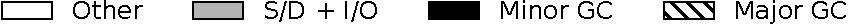
\includegraphics[width=0.5\linewidth]{teraheap/fig/fig23_legend-crop.pdf}
	\\
	\vspace{-11pt}
	\subfloat[Spark-PR]{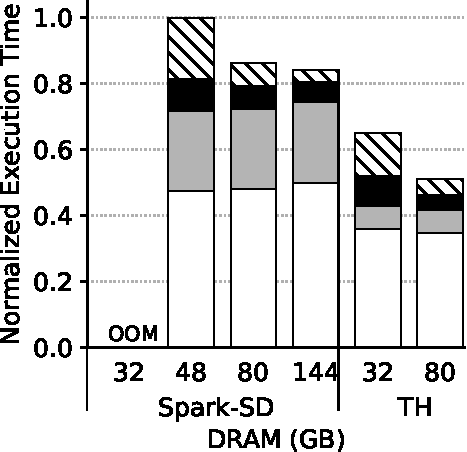
\includegraphics[width=0.19\linewidth]{teraheap/fig/fig10-crop.pdf}}
	\hspace{2pt}
	\subfloat[Spark-CC]{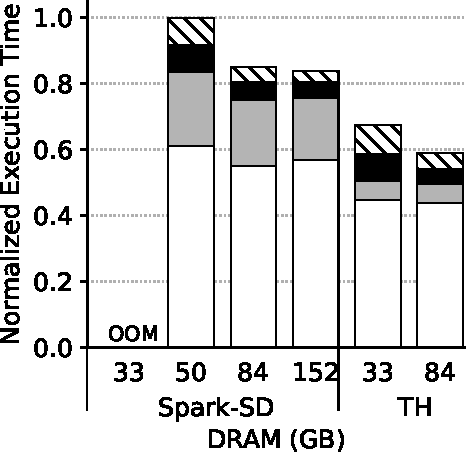
\includegraphics[width=0.19\linewidth]{teraheap/fig/fig11-crop.pdf}}
	\hspace{2pt}
	\subfloat[Spark-SSSP]{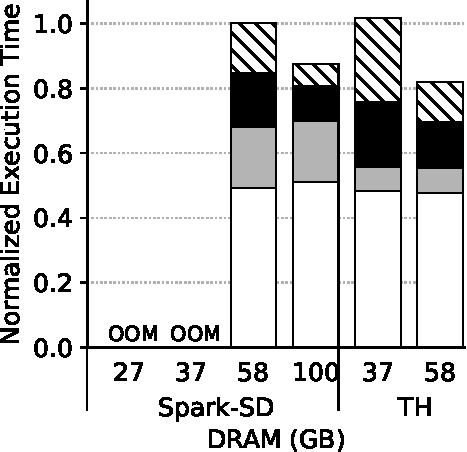
\includegraphics[width=0.19\linewidth]{teraheap/fig/fig12-crop.pdf}}
	\hspace{2pt}
	\subfloat[Spark-SVD]{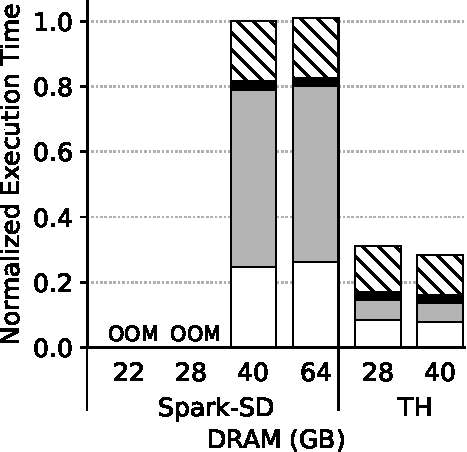
\includegraphics[width=0.19\linewidth]{teraheap/fig/fig22-crop.pdf}}
	\hspace{2pt}
	\subfloat[Spark-TR]{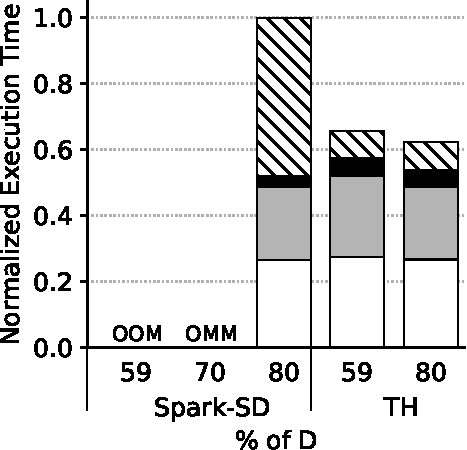
\includegraphics[width=0.19\linewidth]{teraheap/fig/fig23-crop.pdf}}
	\\
	\vspace{-10pt}
  \subfloat[Spark-LR]{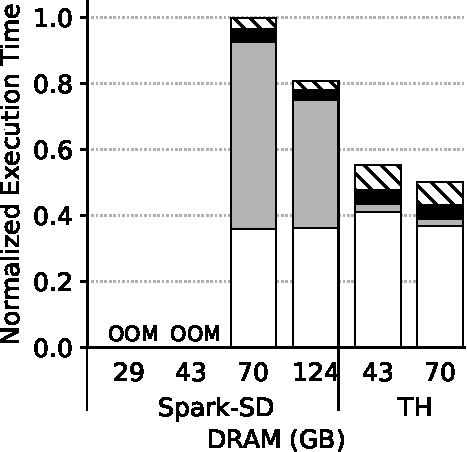
\includegraphics[width=0.19\linewidth]{teraheap/fig/fig26-crop.pdf}}
	\hspace{2pt}
  \subfloat[Spark-LgR]{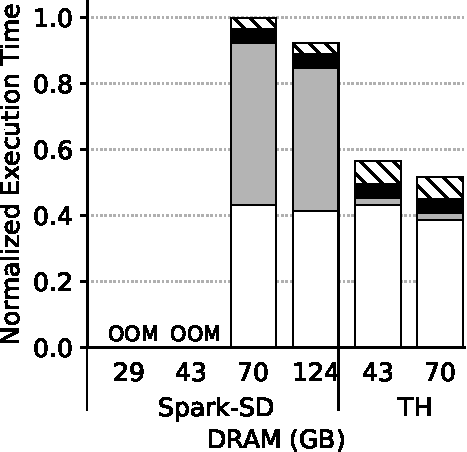
\includegraphics[width=0.19\linewidth]{teraheap/fig/fig27-crop.pdf}}
	\hspace{2pt}
  \subfloat[Spark-SVM]{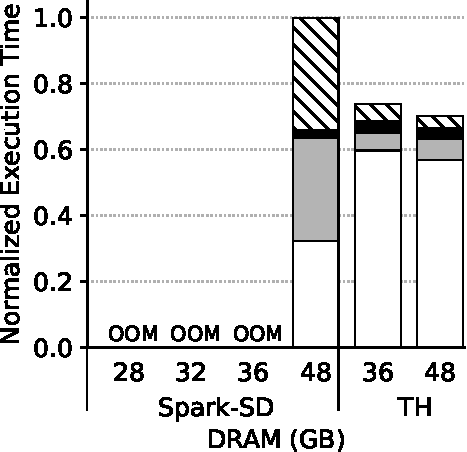
\includegraphics[width=0.19\linewidth]{teraheap/fig/fig28-crop.pdf}}
	\hspace{2pt}
	\subfloat[Spark-BC]{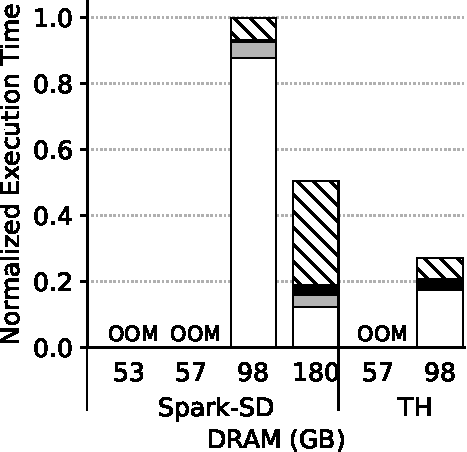
\includegraphics[width=0.19\linewidth]{teraheap/fig/fig29-crop.pdf}}
	\hspace{2pt}
	\subfloat[Spark-RL]{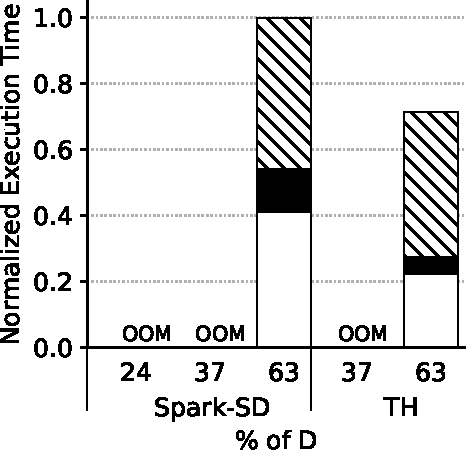
\includegraphics[width=0.19\linewidth]{teraheap/fig/fig30-crop.pdf}}
	\\
	\vspace{-12pt}
	\subfloat[Giraph-PR]{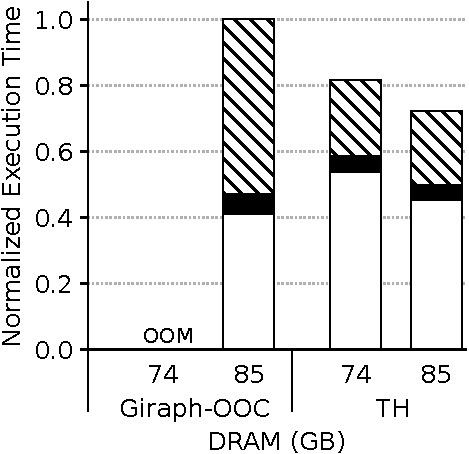
\includegraphics[width=0.19\linewidth]{teraheap/fig/fig40-crop.pdf}}
	\hspace{2pt}
	\subfloat[Giraph-CDLP]{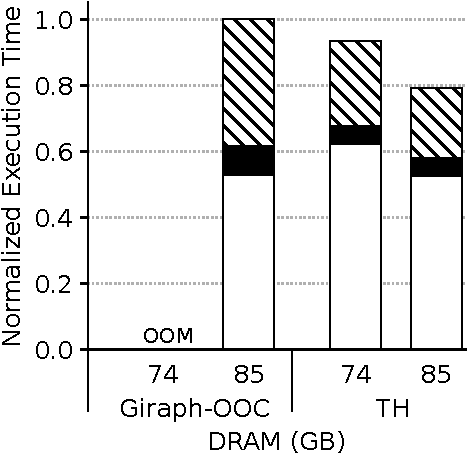
\includegraphics[width=0.19\linewidth]{teraheap/fig/fig41-crop.pdf}}
	\hspace{2pt}
	\subfloat[Giraph-WCC]{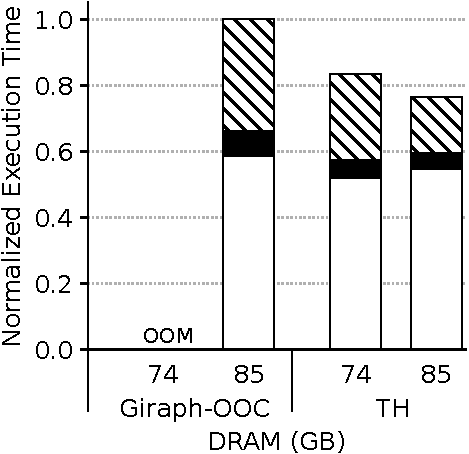
\includegraphics[width=0.19\linewidth]{teraheap/fig/fig42-crop.pdf}}
	\hspace{2pt}
	\subfloat[Giraph-BFS]{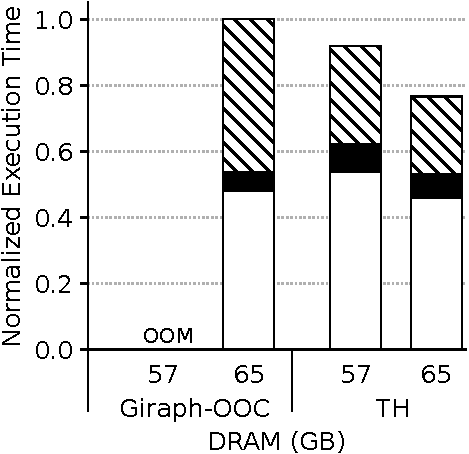
\includegraphics[width=0.19\linewidth]{teraheap/fig/fig43-crop.pdf}}
	\hspace{2pt}
	\subfloat[Giraph-SSSP]{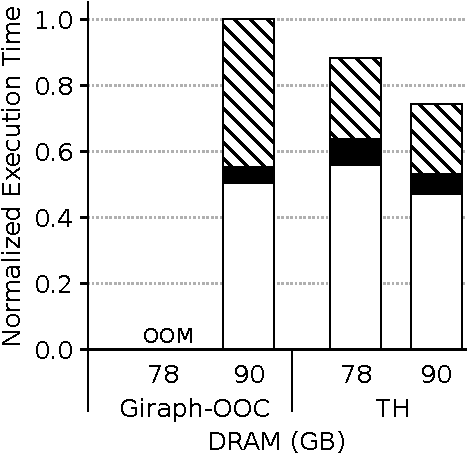
\includegraphics[width=0.19\linewidth]{teraheap/fig/fig44-crop.pdf}}

  \caption{Overall performance of TeraHeap (TH) compared to Spark-SD and
  Giraph-OOC on the NVMe server.}
	\label{fig:dram}
\end{figure*}

First, we investigate the performance benefits of \teraheapName{} under a fixed DRAM
size.
%
Figure~\ref{fig:dram} shows the performance of \teraheapName{} compared to Spark-SD and
Giraph-OOC for the NVMe SSD setup, using OpenJDK17 for Spark and OpenJDK8 for
Giraph.
%
We normalize execution time to the first bar in each figure. Missing bars
indicate out-of-memory (OOM) errors.

Using the same DRAM size, \teraheapName{} reduces execution time in Spark
between 18\% (SSSP) and 73\% (BC) compared to Spark-SD. In Giraph,
\teraheapName{} reduces execution time between 21\% (CDLP) and 28\% (PR). In
both cases, the performance improvement results from reducing the \teraheapGC
overhead, by up to 96\% and 54\% in Spark and Giraph, respectively.
This overhead occurs mainly because cached objects in Spark and
messages and edges in Giraph occupy almost half of the heap,
triggering \teraheapGC more frequently. \teraheapName{} transfers objects to H2,
stressing H1 less.

In addition, \teraheapName{} reduces \teraheapSD cost in Spark-SD, between 2\% (BC)
and 93\% (LR), as it provides direct access to deserialized objects in
H2. Note that \teraheapSD cost in TR and BC for \teraheapName{} is similar to
Spark-SD because the cached data fits in the on-heap cache. In Giraph,
the impact of \teraheapName{} on \teraheapSD overhead (part of other) is minimal
because Giraph serializes objects in the managed heap as well, and not
only as part of moving objects off-heap. Also, in LR, LgR, and SVM
other time with \teraheapName{} increases by up to 43\% compared to Spark-SD.
These workloads perform streaming access on elements of cached RDDs in
each iteration of the ML training phase, which is the largest part of
the execution (100 iterations). Thus, they do not exhibit locality in
the I/O page cache, fetching data from the storage device during the
computation. The average read throughput in these workloads is
\SI{2.9}{GB/s}, which is the peak device read throughput. Using more
NVMe SSDs can reduce other time for LR, LgR, and SVM.

\begin{figure}[t]
	\centering
	\vspace{-8pt}
	\subfloat[Spark-SD]{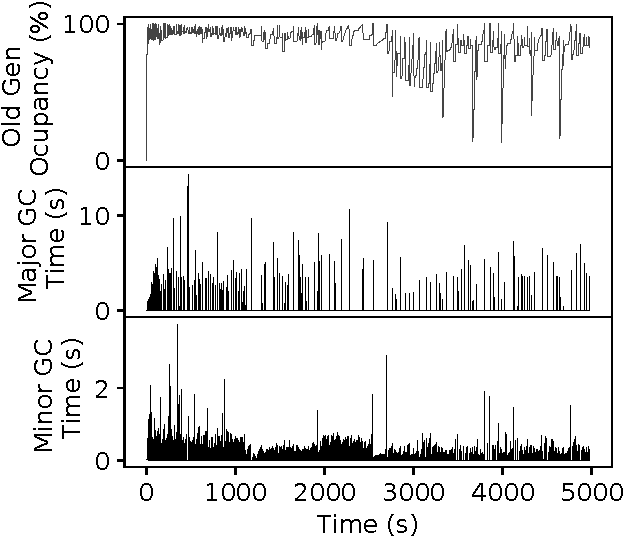
\includegraphics[width=0.4\linewidth]{teraheap/fig/pr_sd_jstat-crop.pdf}}
	\hspace{1pt}
	\subfloat[TeraHeap]{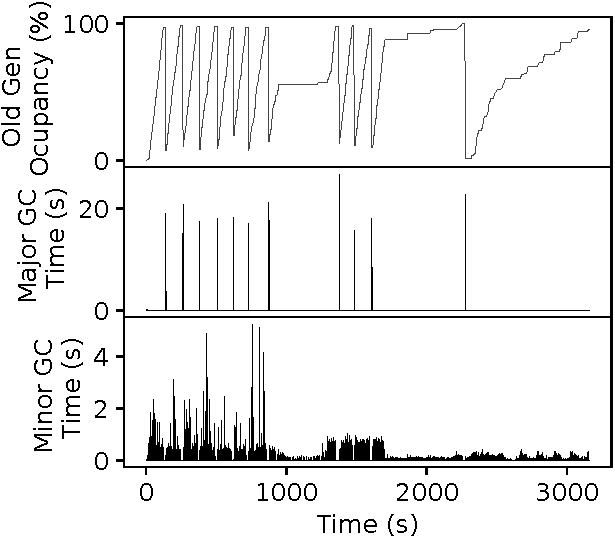
\includegraphics[width=0.4\linewidth]{teraheap/fig/pr_tc_jstat-crop.pdf}}
	\vspace{-0.2\baselineskip}
	\caption{\teraheapGC time and old generation occupancy in PR for (a) Spark-SD
    and (b) TeraHeap. The heap size is 64\:GB.}
	\label{fig:jstat}
\end{figure}

To examine pressure on the managed heap, Figure~\ref{fig:jstat} shows
\teraheapGC behavior for PR with Spark-SD and \teraheapName{} with a \SI{64}{GB} heap. We
examine the execution time for each minor and major \teraheapGC cycle and
monitor the percentage of the old generation consumed by cached
objects. We note that Spark-SD suffers from frequent major \teraheapGC cycles.
There are 171 major \teraheapGC cycles, each requiring, on average, \SI{3.7}{s}.
Each cycle in Spark-SD reclaims 10\% of the old generation objects
(0-\SI{3000}{s} in Figure~\ref{fig:jstat}), as the remaining objects are
live cached objects. However, \teraheapName{} performs only 13 major \teraheapGC
cycles. Each cycle in \teraheapName{} takes, on average, \SI{16}{s}. More than 70\%
is due to I/O during the compaction phase of major \teraheapGC. Finally,
moving objects directly from the young generation to H2 reduces total
minor \teraheapGC time by 38\% compared to Spark-SD. This reduction is because
\teraheapName{} scans fewer cards that track old-to-young references than
Spark-SD.

To illustrate the potential for eliminating \teraheapSD without increasing
\teraheapGC overhead, Figure~\ref{fig:analysis} shows the RDD access patterns
for PageRank (PR) and Connected Components (CC). In our experiments,
each RDD has 256 partitions. The horizontal axis shows time (seconds),
and the vertical axis shows the IDs of accessed RDD partitions (from 1
to maximum partition ID for each RDD). For each ID, the first dot
marks the time when that partition is cached. Each subsequent dot
represents access to this partition by the application.

\begin{figure}
\subfloat[PageRank]{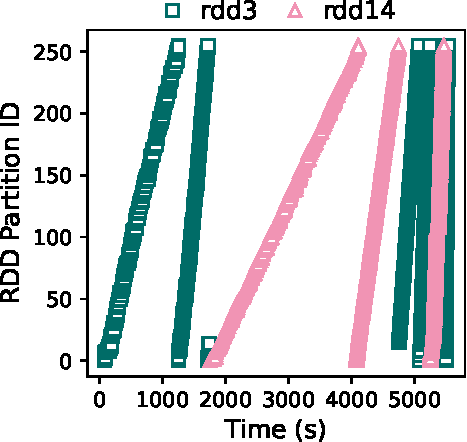
\includegraphics[width=0.37\linewidth]{teraheap/fig/access_pattern/pr_acc_pattern-crop.pdf}}
\hspace{10pt}
\subfloat[Connected Components]{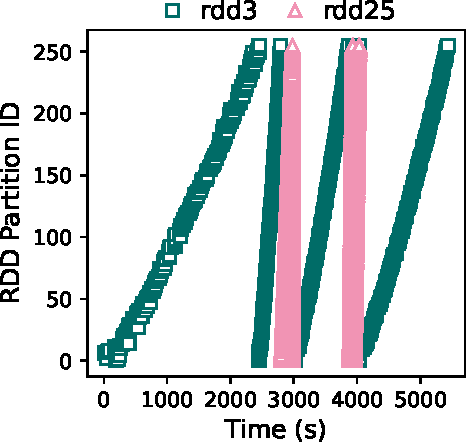
\includegraphics[width=0.37\linewidth]{teraheap/fig/access_pattern/cc-crop.pdf}}
\caption{Analysis of cached RDD accesses in PageRank (PR) and
Connected Components (CC).}
\label{fig:analysis}
\end{figure}

Once Spark needs an RDD for computation, it tends to access all
partitions of an RDD sequentially. For this reason, in
Figure~\ref{fig:analysis}, RDD accesses form ``lines'' and large
intervals exist between accesses to RDD partitions. For example, in PR
and CC, Spark accesses the first partition of RDD3 on its creation
around $T = 0$\:s but then again only after at least 1500\:s (PR) and
2500\:s (CC), respectively. We observe similar temporal gaps between
accesses to RDD14 (PR) and RDD25 (CC) partitions. For certain RDDs,
each partition is potentially accessed multiple times. For instance,
for RDD25, each partition is accessed twice around $T = 3000$\:s.
However, there is still a significant period of inactivity (about
1000\:s) until the next set of accesses around $T = 4000$\:s.
Occasionally, successive accesses to the same partition exhibit
temporal locality because two jobs take turns to cache and materialize
partitions. For example, at $T = 1100$\:s, Job0 creates and caches the
last partition of RDD3, and then Job1 materializes this partition at
$T = 1200$\:s. Overall, the time interval between accesses to each
partition varies between 100-1500\:s in both applications. This
behavior allow us to place cached RDDs (unlike temporary, short-lived
RDDs) on storage devices (off-heap) that offer high capacity.

Furthermore, data objects in each partition have similar lifetime.
When applications \emph{unpersist} an RDD, Spark drops all RDD
partitions from its cache. At this point, in most cases, no references
exist to the corresponding JVM objects. This observation reveals an
opportunity to reclaim cached objects en masse by organizing the
compute cache in groups of data objects with similar lifetimes.

\subsection{\textbf{Reducing DRAM Capacity Demands}}
We examine the potential benefit of \teraheapName{} in reducing DRAM capacity
demands in Figure~\ref{fig:dram}. Using between $1.3\times$ and
$4.6\times$ less DRAM, \teraheapName{} outperforms by up to 65\% (SVD) compared
to Spark-SD. In Giraph, \teraheapName{} with $1.2\times$ less DRAM improves
performance between 7\% (CDLP) and 18\% (PR). For example, using
\teraheapName{} in Giraph-PR, the heap usage in the first phase of the
application (0-\SI{330}{s}) is between 70\% and 100\%. Then, at the end of
the fifth major \teraheapGC, \teraheapName{} reduces heap usage to 13\% because it
moves \SI{17}{GB} of objects to H2. By reducing memory pressure in H1,
\teraheapName{} with less DRAM can provide similar or higher performance than
Spark-SD and Giraph-OOC.

\subsection{Effectiveness of TeraHeap for In-Memory Frameworks}

This section evaluates \teraheapName{} with GDS library in Neo4j using OpenJDK17. We aim
to show that \teraheapName{} can be effective with analytics frameworks written for
in-memory operations only. Unlike Spark and Giraph, GDS requires keeping all the
graph data in memory and not offloading part of the graph off-heap. For this
purpose, we compare \teraheapName{} with two possible approaches that GDS can use today
by enabling the OpenJDK to:
%
(1) allocate the managed heap on an NVMe SSD (GDS-Heap) and
%
(2) allocate only the old generation over NVMe SSD (GDS-OldGen).
%
Figure~\ref{fig:neo4j}(a) shows our results.

\begin{figure}[t]
	\centering
	\subfloat[]{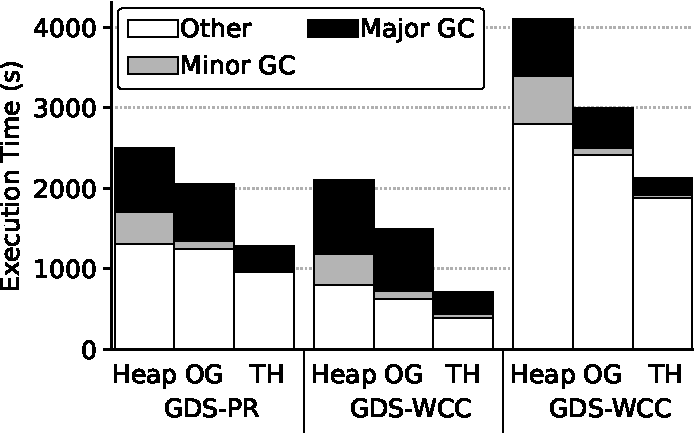
\includegraphics[width=0.4\linewidth]{teraheap/fig/neo4j_pr-crop.pdf}}
  \hspace{10pt}
	\subfloat[]{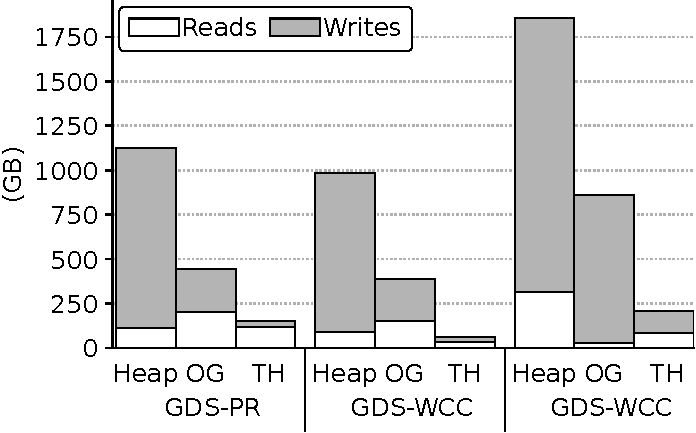
\includegraphics[width=0.4\linewidth]{teraheap/fig/neo4j_io_pr-crop}}
  \caption{(a) Performance and (b) device I/O traffic of GDS with three
    configurations: TeraHeap (TH), native with the full heap mapped to a device
  (Heap), and native with the old generation mapped to a device (OG).}
	\label{fig:neo4j}
\end{figure}

\begin{figure}[t]
	\centering
	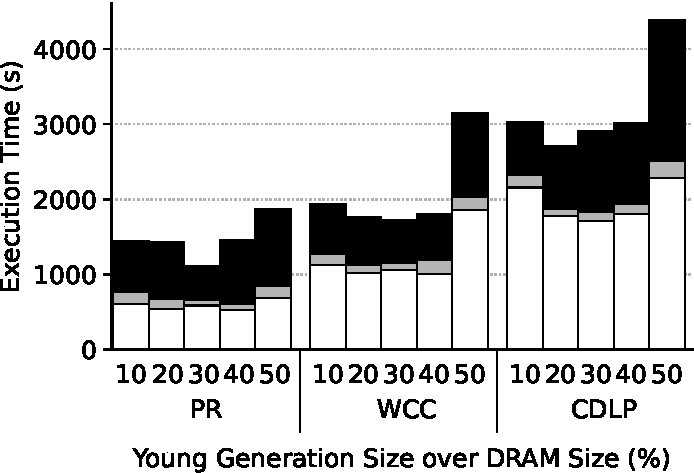
\includegraphics[width=0.5\linewidth]{teraheap/fig/neo4j_oldgen_sensitivity_analysis-crop.pdf}
  \caption{Sensitivity analysis for the size of the young generation over the
    total DRAM size. As the young generation's size increases, the old generation's
  page cache, which is memory-mapped over NVMe SSD, decreases.}
	\label{fig:neo4j_mmap_oldgen}
\end{figure}

Our experiments show that executing applications using GDS-Heap approach
increases execution time between 43\% and 63\% compared to using \teraheapName{}.
Although DRAM is used as a large page cache in this approach, the JVM cannot
control where each object is placed (page cache or storage), and therefore it
does not avoid expensive \teraheapGC scans. Instead, the OS decides which pages to write
to the device and which pages to keep in the page cache based on an LRU policy.
Placing arbitrary objects in the storage device increases minor \teraheapGC time by up
to 91\% compared to \teraheapName{}. This increase in time is because the application
reads and updates young objects over the device. Using \teraheapName{}'s approach of
using two separate heaps to avoid GC in the storage device is essential for
maintaining performance.

On the other hand, \teraheapName{} still outperforms between 21\% and 26\% compared to
GDS-OldGen. Minor \teraheapGC time decreases when allocating the entire heap over the
storage device. However, increasing the young generation's size in DRAM reduces
the page cache size for the objects in the old generation. As we see, there is
no sweet spot for the division of DRAM between the young generation and the
page cache for the old generation.

Figure~\ref{fig:neo4j}(b) depicts the read and write traffic to the storage
device of \teraheapName{} compared to mapping the full heap over the storage device and
mapping only the old generation over the storage device. Overall, \teraheapName{}
reduces I/O traffic by up to 93\% (WCC) compared to both approaches. When the
young generation is in DRAM reduces the I/O traffic compared to allocating the
entire heap over the storage device because it absorbs the read and writes to
young objects in DRAM. Notably, in configurations where the young generation
constitutes 80\% of the total DRAM (Figure~\ref{fig:neo4j_mmap_oldgen}), there
is an increase in read traffic due to the limited size of the page cache
(\SI{3}{GB} for PR and WCC, and \SI{6}{GB} for SSSP, respectively). The size of
the page cache directly impacts accesses to objects in the old generations by
mutator threads, the major \teraheapGC time, and the minor \teraheapGC time involved in updating
references from objects in the old generation to those in the young generation.

\subsection{Effects of Transfer Hint and Low Threshold}
\label{sec:hints}

This section examines the performance effect of using the transfer
hint \texttt{h2\_move()}. Figure~\ref{fig:api}(a) shows the
performance of \teraheapName{} with and without using \texttt{h2\_move()}.
Frameworks use \texttt{h2\_move()} to advise \teraheapName{} when to move
objects with a specified label to H2. Note that in case of high memory pressure,
\teraheapName{} moves to H2 all marked objects without waiting for
\texttt{h2\_move()} hints. Given that \teraheapName{} can use only the high
threshold mechanism to decide when to move objects to H2, we explore
eliminating \texttt{h2\_move()}. This results in objects staying
longer in H1. With a high threshold of 85\%, we see
(Figure~\ref{fig:api}(a)) that using \texttt{h2\_move()} improves
\teraheapName{} performance between 29\% (SSSP) and 55\% (WCC) compared to not
using the hint. In WCC, using \texttt{h2\_move()}, we move objects to
H2 on average every \SI{215}{s}, reducing \teraheapGC cost by 39\% compared to not
using the transfer hint, which transfers objects on average every
\SI{485}{s}. Moving objects with frequent updates to H2 increases
other time by up to 59\% (WCC) due to the large cost of
read-modify-write operations on an I/O device. This increases device
traffic by up to 98\% (writes) due to page-based accesses to the
device. Thus, using the transfer hint is necessary to delay
moving objects with frequent updates to H2 until they become
immutable.

\begin{figure}[t]
	\centering
	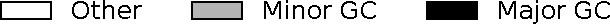
\includegraphics[width=0.45\linewidth]{teraheap/fig/fig47legend-crop.pdf}
	\\
	\vspace{-12pt}
	\subfloat[Effect of transfer hint]{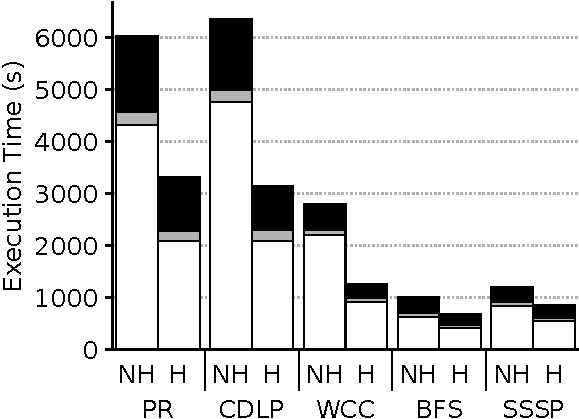
\includegraphics[width=0.4\linewidth]{teraheap/fig/fig47-crop.pdf}}
  \hspace{15pt}
	\subfloat[Effect of low threshold]{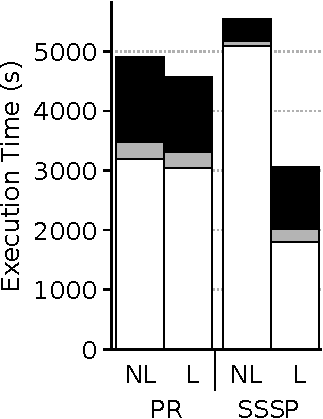
\includegraphics[width=0.24\linewidth]{teraheap/fig/fig48-crop.pdf}}
	\caption{TeraHeap performance for Giraph (a) with (H) and without
		(NH) transfer hint, and (b) with (L) and without (NL) low transfer threshold.}
	\label{fig:api}
\end{figure}

Next, we study how effective is the \teraheapName{} low threshold mechanism.
Figure~\ref{fig:api}(b) shows \teraheapName{} performance using
\texttt{h2\_move()} with and without a low threshold. We use a low
threshold of 50\% (and we leave the high threshold to 85\%). \teraheapName{}
will move objects until it reduces H1 usage to 50\%. We use PR and
SSSP with a large dataset (\SI{91}{GB}) in Giraph. These two workloads
trigger the high threshold mechanism. We use \SI{170}{GB} DRAM and \SI{200}{GB}
DRAM in PR and SSSP, respectively. The percentage of DR1 over total
DRAM is similar to the corresponding workload in
Figure~\ref{fig:api}(a).

Using a low transfer threshold improves \teraheapName{} performance by up to
44\% (SSSP), compared to using only the transfer hint with the high
threshold. For example, in SSSP, during graph loading, we detect high
memory pressure in the fourth major \teraheapGC. After the fourth major \teraheapGC,
most objects in H1 are related to marked edges. Then, in the fifth
major \teraheapGC, we move \SI{44}{GB} of marked objects to H2, reducing H1 usage to
50\%. Therefore, the low transfer threshold reduces read-modify-write
operations on the device by up to 95\%, decreasing the other
time by up
to 65\%. Although there may be benefits in setting the low and high
thresholds dynamically, we leave this for future work.

\subsection{Storage Capacity Consumption}
\label{sec:overhead}

\begin{table}[]
  \centering
    \caption{Metadata size per TB of H2 space.}
  \resizebox{0.6\columnwidth}{!}{%
    \begin{tabular}{l|ccccccccc}
      \multicolumn{1}{l|}{\textbf{Region Size (MB)}}  &   1 &   2 &   4 &  8 & 16 & 32 & 64 & 128 & 256 \\ \hline
      \textbf{MetaData Size (MB)}& 417 & 209 & 104 & 52 & 26 & 13 &  7 &   3 &   2 \\
    \end{tabular}%
    }
    \label{tab:dram}
\end{table}

\begin{figure}[t]
	\centering
  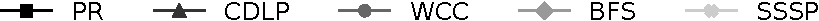
\includegraphics[width=0.5\linewidth]{teraheap/fig/allocator_legend-crop.pdf}
  \vspace{-8pt}
  \\
  \subfloat[Region size = 16\:MB]{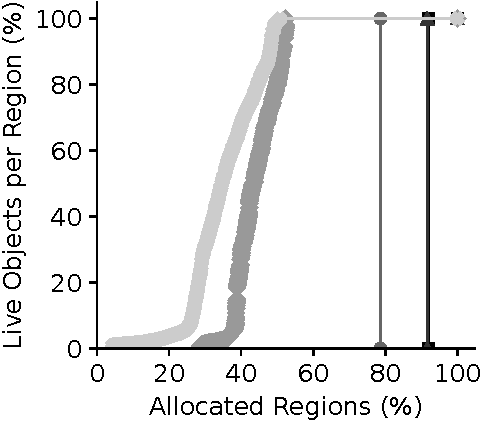
\includegraphics[width=0.23\linewidth]{teraheap/fig/allocator_live_cdf_16-crop.pdf}}
  \hspace{1pt}
  \subfloat[Region size = 256\:MB]{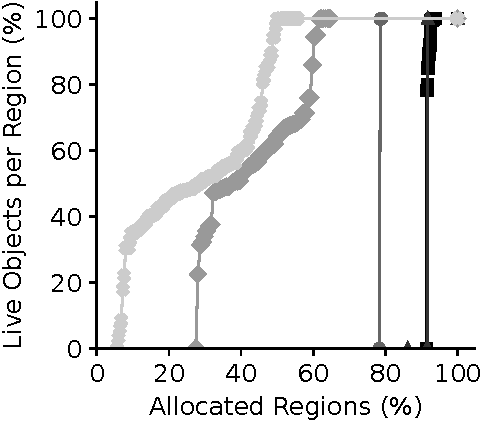
\includegraphics[width=0.23\linewidth]{teraheap/fig/allocator_live_cdf_256-crop.pdf}}
  \hspace{1pt}
  \subfloat[Region size = 16\:MB]{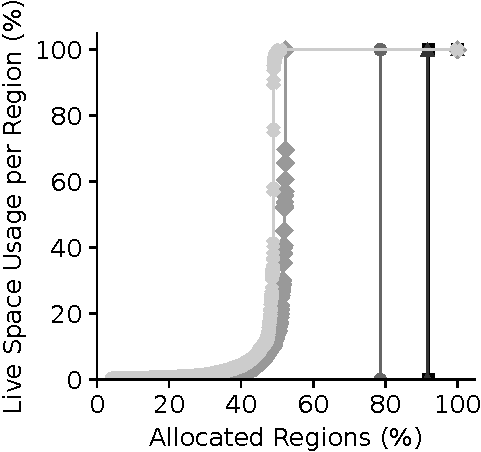
\includegraphics[width=0.23\linewidth]{teraheap/fig/allocator_use_cdf_16-crop.pdf}}
  \hspace{1pt}
  \subfloat[Region size = 256\:MB]{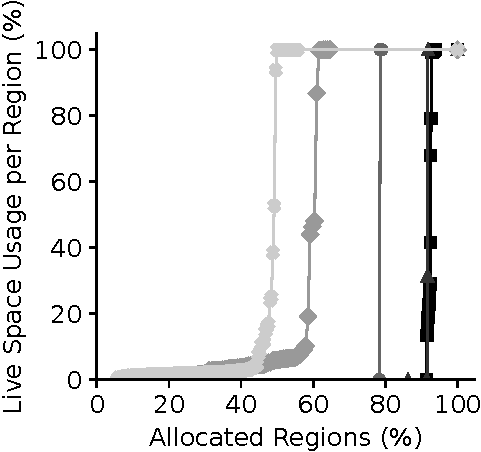
\includegraphics[width=0.23\linewidth]{teraheap/fig/allocator_use_cdf_256-crop.pdf}}
  \caption{
    CDF of the percentage of live objects (a, b) and space
    occupied by live objects (c, d) during execution.
  }
    \label{fig:alloc_stats}
\end{figure}

This section investigates the storage requirements of H2. \teraheapName{}
organizes object groups with a similar lifetime in fixed-size regions
in H2 and reclaims them in bulk. This approach may result in waste of
space for two reasons. First, when the number of objects in a group is
small, unused space in the corresponding region can be large. Second,
one live object can keep the entire region alive, preventing \teraheapName{}
from reclaiming it. Generally, a smaller region size reduces both of
these factors at the cost of increasing metadata in DRAM.

We first show how the region size affects the metadata size for H2.
Table~\ref{tab:dram} shows the metadata size in DRAM per TB of H2, for
region sizes between \SI{1}{MB} and \SI{256}{MB}. As we increase the region size
from \SI{1}{MB} to \SI{256}{MB}, the total metadata in DRAM decreases from
\SI{417}{MB} to \SI{2}{MB}.

Figures~\ref{fig:alloc_stats}(a) and~\ref{fig:alloc_stats}(b) show the
CDF of the percentage of live objects per region for \emph{all
allocated} regions with \SI{16}{MB} and \SI{256}{MB} size, respectively.
Figures~\ref{fig:alloc_stats}(c) and~\ref{fig:alloc_stats}(d) show the
CDF of the percentage of space occupied by live objects for \SI{16}{MB} and
\SI{256}{MB} regions. The number of allocated regions is equal to the sum
of reclaimed regions during execution and the active regions before
JVM shutdown. Although not shown in these figures, we observe in our
measurements that unused space is between 1\% and 3\% for all
workloads in both region sizes. Essentially, \teraheapName{} is able to use
the space in each region it allocates with its append-only placement.

In Figures~\ref{fig:alloc_stats} (a) and~\ref{fig:alloc_stats}(b) all
regions with 0\% live objects are reclaimed during execution. We see
that in PR, CDLP, and WCC, \teraheapName{} reclaims most allocated regions and
around 90\% in CDLP and PR for both region sizes.  In BFS and SSSP,
\teraheapName{} reclaims 28\% and 6\% of the total allocated regions,
respectively. In BFS and SSSP, although most of the objects in a
region are live, most of the space is occupied by large dead arrays.
For example, in SSSP with \SI{256}{MB} regions, in 90\% of the regions at
least 20\% of the objects are live. However, in 45\% of the regions,
the live objects occupy less than 10\% of the allocated region space
(Figure~\ref{fig:alloc_stats}(d)). In these cases, using \SI{16}{MB}
regions is more appropriate because they reduce by 10\% (BFS) the
space waste compared to \SI{256}{MB} regions. We believe that future work
can investigate object placement policies for H2 that takes into
account object size to further improve space efficiency on storage
devices.

\begin{figure}[t]
	\centering
	\subfloat[]{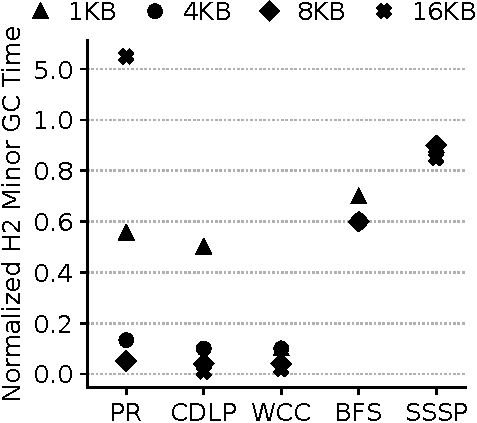
\includegraphics[width=0.3\linewidth]{teraheap/fig/fig4-crop.pdf}}
  \hspace{20pt}
	\subfloat[]{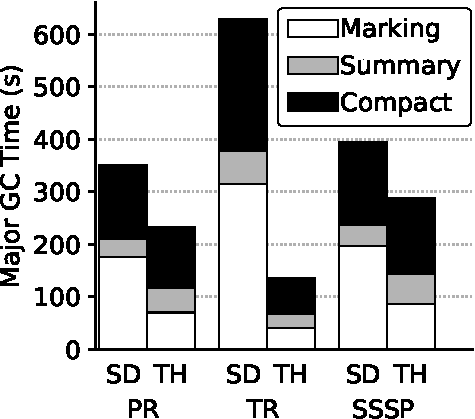
\includegraphics[width=0.3\linewidth]{teraheap/fig/fig5-crop.pdf}}
	\caption{(a) Minor \teraheapGC time in H2 for different card segment sizes
    using a 256\:MB stripe size in Giraph. (b) Major \teraheapGC time using
  Spark-SD (SD) and TeraHeap (TH).}
	\label{fig:gc}
\end{figure}


\subsection{\teraheapGC Overhead}
The garbage collector in \teraheapName{} performs additional work during minor
\teraheapGC that involves scanning H2 cards and updating backward references.
We evaluate this overhead for different card segment sizes in Giraph.
Figure~\ref{fig:gc}(a) shows minor \teraheapGC time in H2 for \SI{1}{KB}, \SI{4}{KB},
\SI{8}{KB}, and \SI{16}{KB} card segments, normalized to \SI{512}{B} card segments.
We see that increasing the size of card segments from \SI{512}{B} to \SI{16}{KB}
reduces minor \teraheapGC time on average by $64\%$. Larger card segments
result in a smaller card table, and less time is required to scan the
respective cards. However, increasing card segment size increases the
cost of scanning each card segment if the respective card is marked as
dirty. For example, increasing the card segment size in PR  from
\SI{512}{B} to \SI{16}{KB} leads to an increase in minor \teraheapGC time for scanning
and updating H2 objects with backward references (H2 to H1) by
$5\times$. In Spark, updates to H2 objects are infrequent compared to
Giraph, as RDDs are immutable.

Next, we examine the overheads introduced by \teraheapName{} during major \teraheapGC for H1 by
moving objects to H2, which involves device I/O when using SSDs as the backing
device. Figure~\ref{fig:gc}(b) shows the three phases of major \teraheapGC time using
Spark-SD and \teraheapName{}. Overall, \teraheapName{} improves marking and compaction phases of
major \teraheapGC by up to 87\% (PR) compared to Spark-SD because we avoid scanning H2
objects. For example, in PR, the collector avoids following in each GC, on
average, 95 million forward references from H1 to H2 objects. The summary phase
takes up to 20\% of the major \teraheapGC time as it needs to scan the bitmap, which
indicates H2 candidates and assigns them an H2 address to move during
compaction. In contrast, in native PS, the summary phase is much faster, as it
simply assigns each region of H1 a destination address, eliminating the need for
scanning individual objects. We note that the compaction phase takes 50\% of the
major \teraheapGC time in \teraheapName{} due to the device I/O. We should note that the
overhead of reclaiming H2 dead regions accounts up to 2\% of the total major \teraheapGC
cost because we zero only the metadata of each region in DRAM without
introducing any I/O overhead.

\paragraph{\textbf{Size distribution of H2 objects}}
\setlength{\unitlength}{1em}

\begin{table}[t]
  \centering
  \caption{Categorizing H2 objects into size ranges, such
  as B, KB, and MB, showing the total number of objects for each
  category as a percentage over the total allocated objects in H2.}
\resizebox{\columnwidth}{!}{%
\begin{tabular}{lrrrrrrrrrr|rrrrr}
  \toprule
            & \multicolumn{10}{c|}{\textbf{Spark}}                                             & \multicolumn{5}{c}{\textbf{Giraph}}   \\
 &
  \multicolumn{1}{c}{\textbf{PR}} &
  \multicolumn{1}{c}{\textbf{CC}} &
  \multicolumn{1}{c}{\textbf{SSSP}} &
  \multicolumn{1}{c}{\textbf{SVD}} &
  \multicolumn{1}{c}{\textbf{TR}} &
  \multicolumn{1}{c}{\textbf{LR}} &
  \multicolumn{1}{c}{\textbf{LgR}} &
  \multicolumn{1}{c}{\textbf{SVM}} &
  \multicolumn{1}{c}{\textbf{BC}} &
  \multicolumn{1}{c|}{\textbf{RL}} &
  \multicolumn{1}{c}{\textbf{PR}} &
  \multicolumn{1}{c}{\textbf{CDLP}} &
  \multicolumn{1}{c}{\textbf{WCC}} &
  \multicolumn{1}{c}{\textbf{BFS}} &
  \multicolumn{1}{c}{\textbf{SSSP}} \\
  \toprule
  \textbf{B (\%)}  & 87.51 & 50.36 & 99.33 & 100.00 & 80.33 & 60.20 & 93.80 & 60.61 & 100.00 & 100.00 & 83.44 & 81.41 & 82.92 & 82.33 & 73.32 \\
  \textbf{KB (\%)} & 10.95 & 48.40 & 0.66  & 0.00   & 19.54 & 0.00  & 0.00  & 0.00  & 0.00   & 0.00   & 16.56 & 18.59 & 17.08 & 17.67 & 26.68 \\
  \textbf{MB (\%)} & 1.54  & 1.24  & 0.01  & 0.00   & 0.13  & 39.80 & 6.20  & 39.39 & 0.00   & 0.00   & 0.00  & 0.00  & 0.00  & 0.00  & 0.00  \\
  \bottomrule
\end{tabular}%
}
\label{tab:size}
\end{table}

Next, we examine the size of the objects in H2 to understand how
object size affects device I/O traffic when moving objects from H1
to H2. Table~\ref{tab:size} categorizes H2 objects into size ranges,
such as B, KB, and MB, showing the total number of objects for each
category as a percentage of the total allocated objects in H2. In all
the workloads, both Spark and Giraph, the size of the majority of the
objects (up to 100\%) are in the order of bytes. Although Giraph
avoids using objects in the order of MBs, 39\% of the objects in LR
and SVM are in the order of MB. LR and SVM create large arrays of
objects used in each algorithm iteration. Based on the observation
that most objects are in the order of bytes, we use a promotion buffer
per region in H2 that writes objects to the device in batches,
amortizing the system call overhead.

\subsection{TeraHeap Performance with NVM}
\label{sec:nvm}

Figure~\ref{fig:nvm} shows the performance of Spark-SD, Spark-MO, and \teraheapName{} on
our NVM-based setup. Our goal is to examine the benefits of \teraheapName{} when using
NVM to increase the heap size, which can eliminate \teraheapSD at increased \teraheapGC cost
for native. Figure~\ref{fig:nvm}(a) shows that \teraheapName{} improves performance by
up to 79\% and on average by 56\%, compared to Spark-SD. Unlike the off-heap
cache in Spark-SD, \teraheapName{} allows Spark to directly access cached objects in H2
via load/store operations to NVM, without the need to perform \teraheapSD. \teraheapName{}
significantly reduces \teraheapSD and \teraheapGC time compared to Spark-SD by up to 97\% and
93\%, respectively.

\begin{figure*}[t]
	\centering
	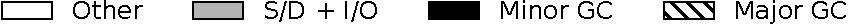
\includegraphics[width=0.5\linewidth]{teraheap/fig/fig9legend-crop.pdf}
	\\
	\vspace{-12pt}
	\subfloat[Spark-SD vs TeraHeap]{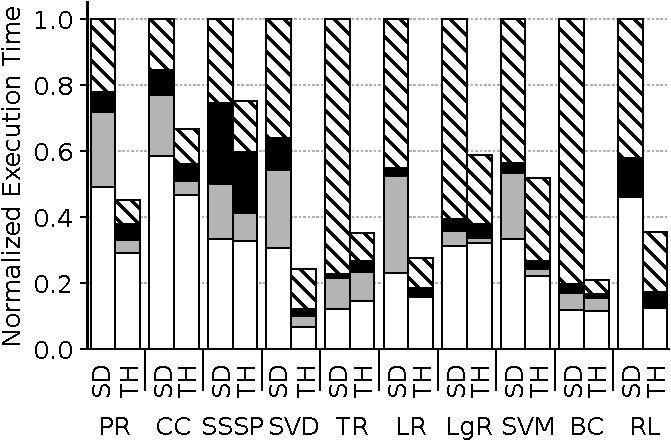
\includegraphics[width=0.32\linewidth]{teraheap/fig/fig9-crop.pdf}}
  \hspace{0.2pt}
	\subfloat[Spark-MO vs TeraHeap]{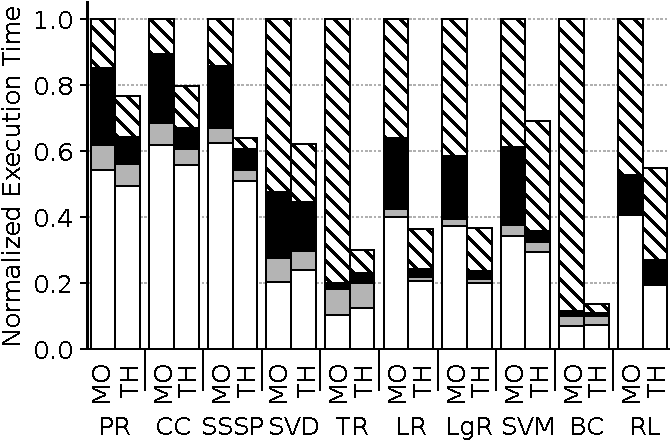
\includegraphics[width=0.32\linewidth]{teraheap/fig/fig9b-crop.pdf}}
  \hspace{0.2pt}
  \subfloat[Panthera vs TeraHeap]{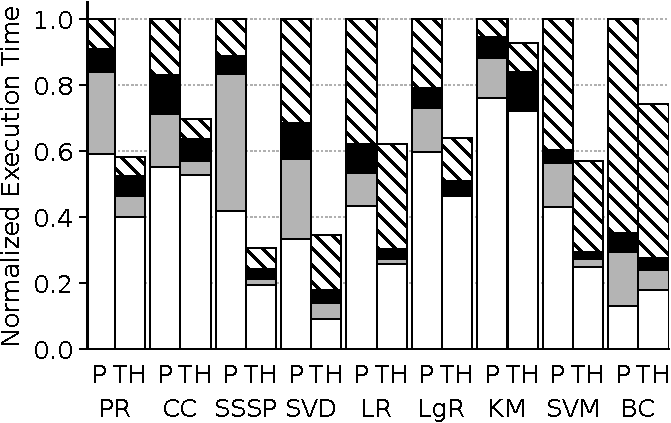
\includegraphics[width=0.32\linewidth]{teraheap/fig/fig25-crop.pdf}}
  \caption{TeraHeap (TH) performance compared to (a) Spark-SD,
		(b) Spark-MO, and (c) Panthera (P) over NVM server.}
	\label{fig:nvm}
\end{figure*}

Figure~\ref{fig:nvm}(b) shows that \teraheapName{} improves performance by up
to 86\% and on average by 48\%, compared to Spark-MO. The main
improvement of \teraheapName{} results from the reduction of minor \teraheapGC and
major \teraheapGC time by up to 88\% (on average by 52\%) and 96\% (on average
by 46\%) compared to Spark-MO, respectively. In Spark-MO, running the
garbage collector on top of NVM (using DRAM as a cache) incurs high
overhead due to the latency of NVM~\cite{izra:nvm} and the agnostic
placement of objects. For instance, minor \teraheapGC time in Spark-MO
increases on average by 36\% compared to Spark-SD
(Figure~\ref{fig:nvm}b) because objects of the young generation are
placed in NVM, resulting in higher access latency for the garbage
collector. Unlike \teraheapName{} that controls object placement in NVM (H2),
Spark-MO relies on the memory controller to move objects between DRAM
and NVM. We measure that Spark-MO incurs on average $5.3\times$ and
$11.8\times$ more read and write operations to NVM compared to
\teraheapName{}, resulting in higher overhead. Therefore, the ability to maintain
separate heaps allows \teraheapName{} to both limit \teraheapGC cost and reduce the
adverse impact of the increased NVM access latency on \teraheapGC time.

We also compare \teraheapName{} with Panthera~\cite{wang:Panthera}\footnote{As
Panthera is not publicly available, we are thankful to the authors for
providing us their code.}, a system designed to use NVM as a heap in
Spark. Panthera extends the managed heap over DRAM and NVM, placing
the young generation in DRAM and splitting the old generation into
DRAM and NVM components. We configure Panthera similar to Wang
\emph{et. al}~\cite{wang:Panthera} with \SI{64}{GB} heap, 25\% on DRAM
(\SI{16}{GB}), and 75\% on NVM. We set the size of the young
generation to $\frac{1}{6}$ (\SI{10}{GB}) of the total heap size and
place it entirely on DRAM. We set the size of the old generation to
the rest of the heap size (\SI{54}{GB}) and place \SI{6}{GB} on DRAM
and the rest (\SI{48}{GB}) on NVM. We configure \teraheapName{} to use an H1
of \SI{16}{GB} and map H2 to NVM. Thus, both systems use the same DRAM
and NVM capacity.

Figure~\ref{fig:nvm}(c) shows that \teraheapName{} improves performance
between 7\% and 69\% compared to Panthera across all workloads.
Panthera bypasses the allocation of some objects in the young
generation, allocating them directly to the old generation. However,
each major \teraheapGC still scans all objects in the old generation, which
increases overhead as the heap address space grows. Instead, \teraheapName{}
reduces the address space that needs to be scanned by the garbage
collector. Note that Panthera incurs more accesses to NVM because it
allocates mature long-lived objects that are highly read and updated
by the mutator threads. Specifically, it increases other by up
to 53\% because it performs more NVM read (up to $54\times$) and NVM
write (up to $51\times$) operations than \teraheapName{}.

\subsection{Performance Scaling}
\label{sec:scaling}

\begin{figure}[t]
	\centering
	\vspace{-5pt}
	\subfloat[Number of mutator
		threads]{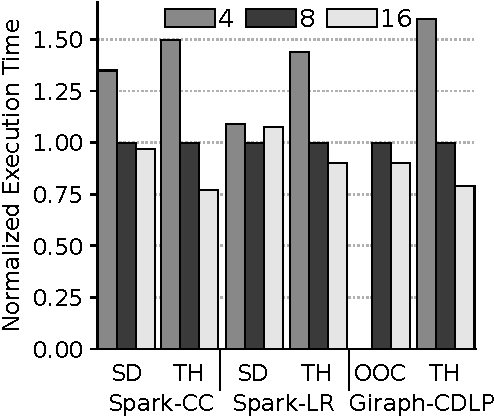
\includegraphics[width=0.3\linewidth]{teraheap/fig/fig49-crop.pdf}}
    \hspace{20pt}
	\subfloat[Dataset size (GB)]{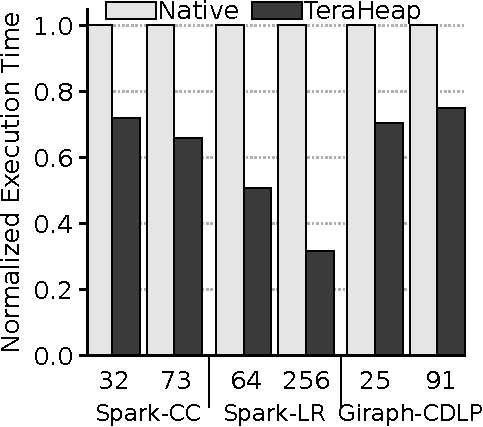
\includegraphics[width=0.3\linewidth]{teraheap/fig/fig46-crop.pdf}}
  \caption{Performance scaling with (a) number of mutator threads and
  (b) dataset size in the NVMe server.}
	\label{fig:scala}
\end{figure}

A benefit of \teraheapName{} is that it allows increasing the number of
mutator threads in Spark and Giraph executors. In both Spark and
Giraph, each mutator thread processes a separate partition. Thus, as
the number of threads in the executor increases, the object allocation
rate increases, leading to higher \teraheapGC{} cost.
Figure~\ref{fig:scala}(a) shows the performance of CC, LR, and CDLP
(other workloads show similar behavior) using Spark-SD, Giraph-OOC,
and \teraheapName{} (TH) with 4, 8, and 16 threads, normalized to 8 threads
per configuration. We note that Giraph-OOC with four threads results
in an OOM error. \teraheapName{} allows applications to scale performance
further to 23\% with $2\times$ more threads. However, Spark-SD does
not scale beyond 8 threads in LR because \teraheapGC{} cost increases (by
44\%), eliminating any benefits from using more threads. We note that
increasing the number of threads in Spark-SD reduces \teraheapSD cost by up
to 55\% (CC) because Spark parallelizes the \teraheapSD process. Although
Giraph-OOC (native) improves performance by 10\% using 16 executor
threads, it still performs $1.4\times$ more major GCs than eight
executor threads. Finally, \teraheapName{} significantly alleviates memory
pressure by moving a large portion of H1 objects to H2, leaving more
room for mutator threads to work without the need for frequent \teraheapGC.

We also investigate the performance benefits of \teraheapName{} for a larger
dataset in Figure~\ref{fig:scala}(b). We observe similar (CDLP) or
higher improvements (CC, LR) compared to the smaller datasets. \teraheapName{}
is robust to different dataset sizes and improves performance by up to
70\% compared to Spark-SD and Giraph-OOC, while our expectation is
that benefit will increase further as dataset size increase.

\subsection{Sensitivity Analysis}

\begin{figure}[t]
	\centering
	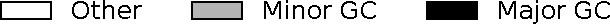
\includegraphics[width=0.45\linewidth]{teraheap/fig/fig47legend-crop.pdf}
	\\
  \subfloat[Giraph-PR]{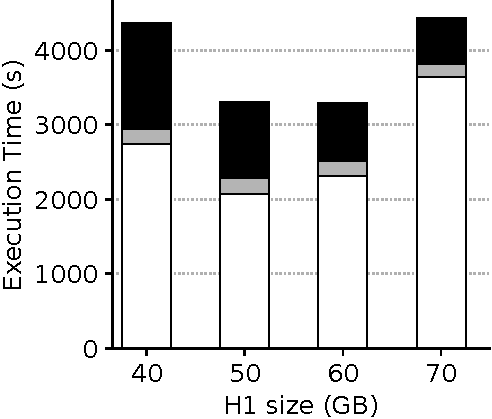
\includegraphics[width=0.2\linewidth]{teraheap/fig/sensitivity_pr-crop.pdf}}
  \subfloat[Giraph-CDLP]{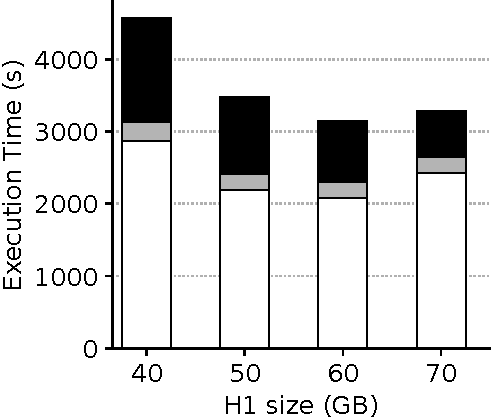
\includegraphics[width=0.2\linewidth]{teraheap/fig/sensitivity_cdlp-crop.pdf}}
  \subfloat[Giraph-WCC]{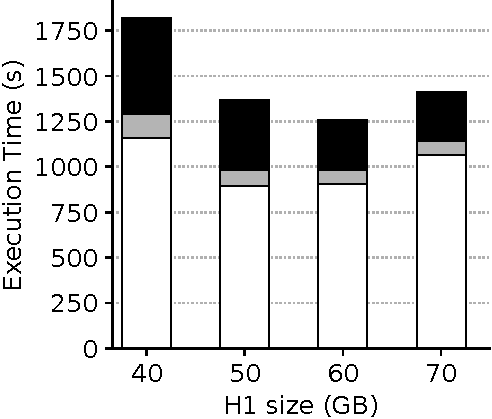
\includegraphics[width=0.2\linewidth]{teraheap/fig/sensitivity_wcc-crop.pdf}}
  \subfloat[Giraph-BFS]{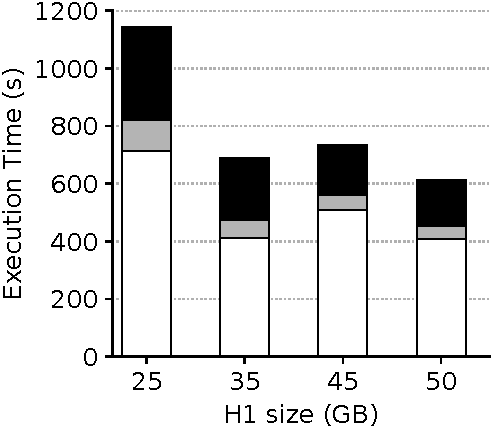
\includegraphics[width=0.2\linewidth]{teraheap/fig/sensitivity_bfs-crop.pdf}}
  \subfloat[Giraph-SSSP]{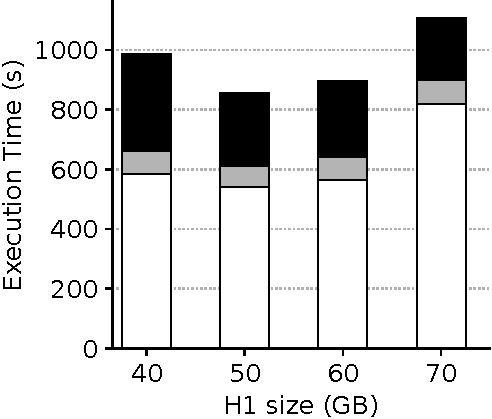
\includegraphics[width=0.2\linewidth]{teraheap/fig/sensitivity_sssp-crop.pdf}}
  \caption{Sensitivity of \teraheapName{} to the size of H1 (relative to the size of
    page cache for H2) with a constant amount of DRAM capacity in NVMe server.}
	\label{fig:sense}
\end{figure}

Next, we examine the sensitivity of \teraheapName{} to dividing a fixed amount of DRAM
between H1 and page cache for H2 in Giraph workloads. Figure~\ref{fig:sense}
shows the performance of \teraheapName{} when H1 varies from \SI{40}{GB} to \SI{70}{GB}
in PR, CDLP, WCC, and SSSP workloads. In BFS, H1 varies from \SI{25}{GB} to
\SI{50}{GB}. Since the DRAM capacity remains constant in all configurations
(\SI{75}{GB} in PR, CDLP, WCC, and SSSP, and \SI{55}{GB} in BFS), the size of
DR2 decreases accordingly. By increasing H1, both minor and major \teraheapGC time
decrease by up to 39\% and 57\%, respectively, because the garbage collector
performs less \teraheapGC cycles. However, the limited size of the page cache (when H1
occupies a large part of the DRAM) affects the accesses to objects in H2,
increasing other time by up to 30\% (SSSP). We note that in WCC, CDLP, and BFS,
using small H1 affects the other time due to the high I/O traffic to the device.
Small H1 size affects the transfer rate of the candidate objects from H1 to H2
because we bypass the transfer hint from the framework. This results in moving
objects to H2 before they become immutable. As a future work, \teraheapName{} could
investigate the dynamic division of DRAM between H1 and page cache for H2 in a
manner that minimizes the sum of the two dominating metrics: \teraheapGC time for H1 and
I/O time for H2.

\begin{figure}[t]
	\centering
	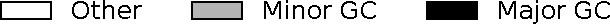
\includegraphics[width=0.45\linewidth]{teraheap/fig/fig47legend-crop.pdf}
	\\
  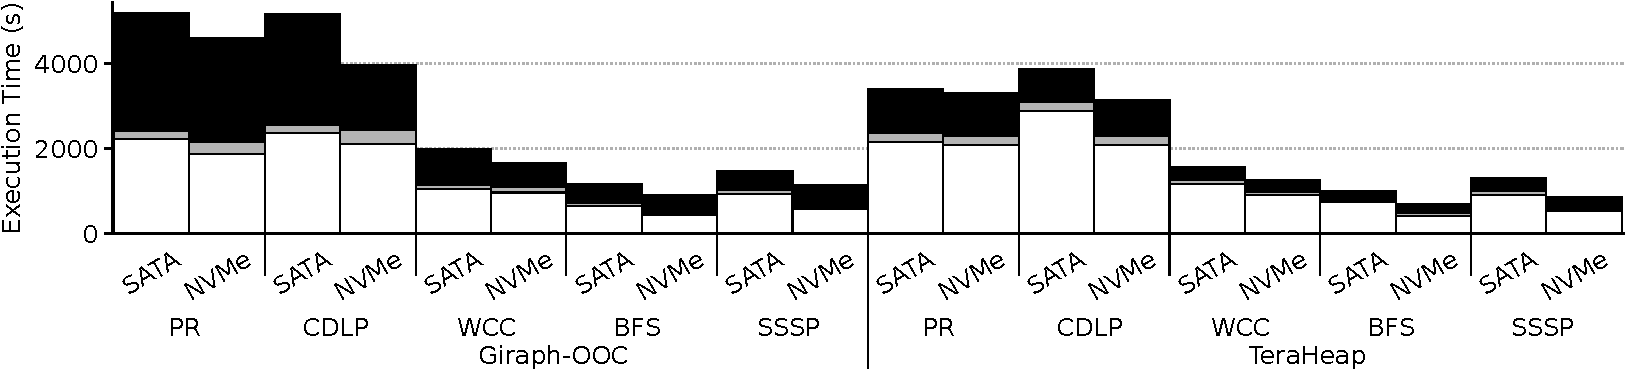
\includegraphics[width=\linewidth]{teraheap/fig/sata_ssd-crop.pdf}
  \caption{Performance of \teraheapName{} compared to Giraph-OOC in
  terms of storage technology.}
	\label{teraheap:fig:sata_ssd}
\end{figure}

Next, we examine the sensitivity of \teraheapName{} compared to storage
devices heterogeneity, allocating H2 over SATA SSD. In our evaluation,
we utilize a RAID 0 configuration of two SATA SSDs. SATA SSDs differ
from NVMe SSDs in terms of interface and speed. NVMe SSDs use the PCIe
interface, which provides faster data transfer speed than SATA SSDs
that use the older SATA interface. Also, the read and write throughput
of our NVMe SSD is $6\times$ and $4\times$ higher compared to SATA
SSD, respectively.

Figure~\ref{teraheap:fig:sata_ssd} shows the performance of \teraheapName{} compared to
Giraph-OOC with OpenJDK8 using NVMe SSD and SATA SSD with the same
amount of DRAM. Despite the use of a slower storage device with SATA
SSD, \teraheapName{} still outperforms Giraph-OOC, improving performance
between 12\% (SSSP) and 34\% (PR). This improvement is mainly due to
reducing major \teraheapGC overhead by up to 71\% (CDLP). Notably, the slower
storage device impacts the performance of \teraheapName{} in terms of object
access by mutator threads and object transfer to H2 during major \teraheapGC.

\subsection{\textbf{Comparison with Newer Garbage Collectors}}
We next present the performance of \teraheapName{} implemented in OpenJDK17
compared to PS and G1 on OpenJDK17. G1 is a generational, region-based
garbage collector which uses concurrent and parallel phases to reduce
pause time and to maintain high \teraheapGC throughput. When G1 determines
that a \teraheapGC is necessary, it collects the regions with the least live
data first (garbage first). Figure~\ref{fig:g1} shows the performance
of Spark with PS, G1, and \teraheapName{}, for the same amount of DRAM.

\teraheapName{} improves performance compared to PS between 5\% (RL)
and 56\% (SVD). The main performance improvement of \teraheapName{} is from
the reduction of \teraheapSD overhead because \teraheapName{} provides direct access
to H2 objects for computation. We note that in RL, the \teraheapName{} major
\teraheapGC time is 36\% higher than that of Spark-SD. This difference is
because a significant portion of the major \teraheapGC time is spent on
performing forwarding table lookups. Before moving objects from H1 to
H2 in RL, we must adjust a subset of H1 objects with 5 million
combined forwarding references to the H2 candidate objects. As
discussed in Section~\ref{teraheap:sec:impl}, future work should examine
alternative approaches beyond forwarding tables.

\begin{figure}[t]
	\centering
	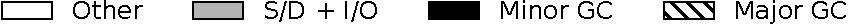
\includegraphics[width=0.6\linewidth]{teraheap/fig/fig9legend-crop.pdf}
	\\
	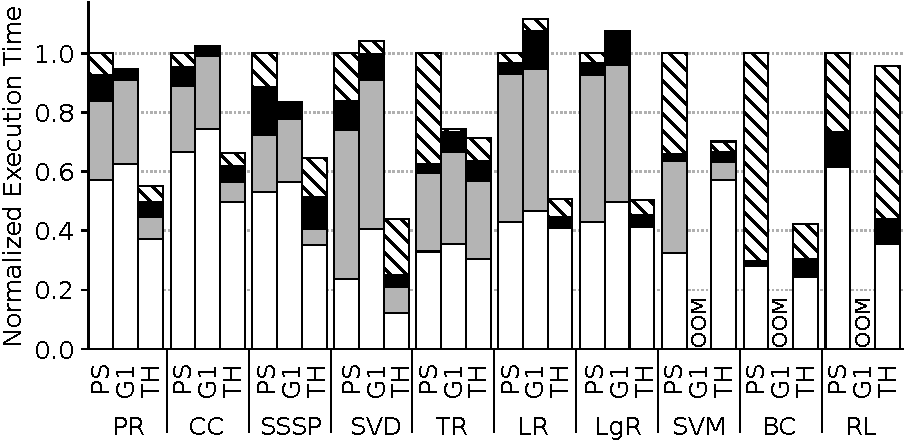
\includegraphics[width=0.7\linewidth]{teraheap/fig/jvm17-crop.pdf}
  \caption{Performance of TeraHeap (TH) compared to native
  execution of Spark-SD on the NVMe server with the Parallel Scavenge
  (PS) and Garbage First (G1) garbage collectors on OpenJDK17.}
	\label{fig:g1}
\end{figure}

On the one hand, G1 outperforms PS in three out of ten workloads
between 5\% (PR) and 25\% (TC) because it reduces \teraheapGC time by up to
95\%. On the other hand, G1 underperforms PS in WCC, SVD, LR, and LGR
between 2\% (WCC) and 12\% (LgR). The source of the slowdown is the
expensive GC post-write barriers that G1 uses. The expensive
post-write barriers increase mutators' threads time (other time).
Also, G1 cannot eliminate the high \teraheapSD (up to 44\%) caused by the
limited DRAM size and the amount of cached data. Unlike G1, \teraheapName{}
eliminates \teraheapSD overhead, providing direct access to the storage
resident objects. Thus, \teraheapName{} improves performance between 4\% (TC)
and 57\% (SVD) compared to G1.

Note that G1 cannot run SVM, BC, and RL due to fragmentation problems
caused by \emph{humongous objects}. Humongous objects in G1 are ones
that are bigger than half of the G1 region size. Such objects are
allocated separately in contiguous regions (humongous regions). A
humongous region can accommodate only one humongous object. The space
between the end of the humongous object and the end of the humongous
region, which in the worst case can be close to half the region size,
is unused. Therefore, when many long-lived humongous objects exist, G1
exhibits significant fragmentation, resulting in OOM errors. PS
resolves fragmentation, performing object compaction when the heap
becomes full.

We note that \teraheapName{} can also be used with G1 to eliminate \teraheapSD cost
and reduce the amount of data subject to \teraheapGC, by moving long-lived,
humongous objects to H2.
